\section{Elaboration of one of the major points of the report}
\begin{verbatim}
 <What follows is example text.>
\end{verbatim}
Investment from operators today is traditionally based on providing connectivity  – providing bandwidth i.e. the “dumb-pipe” \cite{wikibooks-latex}. As the Return of Investment by adding bandwidth declines, operators are searching for new ways for reversing the trend. Their objective is to spend less on running the network while investing in the provisioning of revenue-generating premium services depicted in the Figure~\ref{fig:why}. 

\begin{figure}
	\begin{center}
		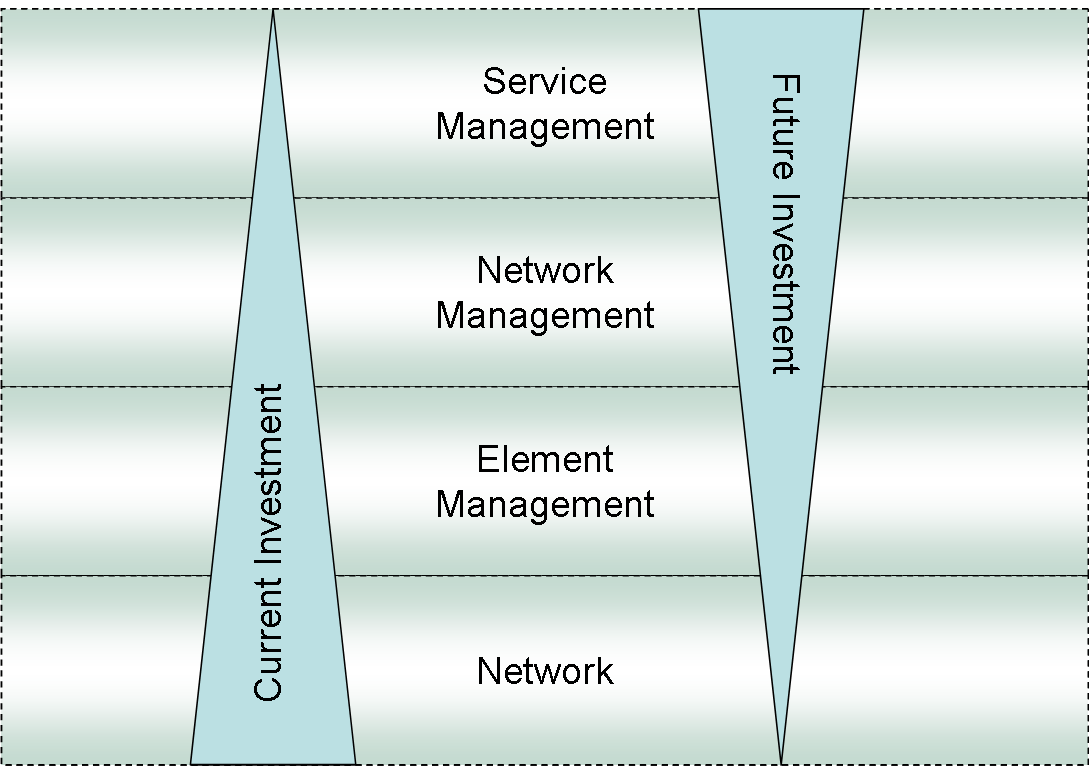
\includegraphics[width=0.8\textwidth]{figures/fig1.png}
		\caption{Why Premium Services?}
		\label{fig:why}
	\end{center}
\end{figure}

For network operators to increase their revenue streams their investment portfolio needs re-positioning. There is a need for greater investment in their services and in particular premium services. Some operators already have made strides in this direction, see Case Study on Portugal Telecom.

However, premium services require service assurance which is to a degree premium management.

To achieve this re-positioning of investment current OPEX levels must be reduced by operators. A number of mechanisms are available to operators in order to achieve this.

\begin{figure}
	\begin{center}
		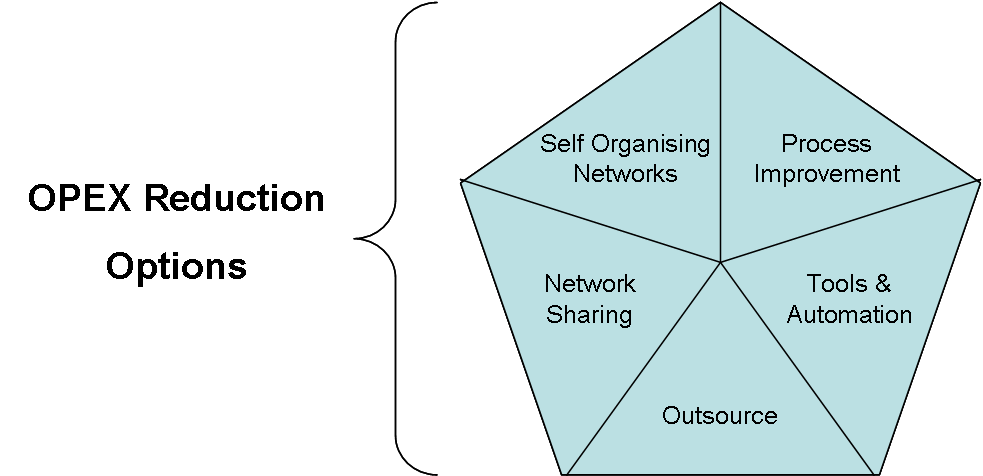
\includegraphics[width=0.8\textwidth]{figures/fig2}
		\caption{Methods for Reducing OPEX}
		\label{fig:opex}
	\end{center}
\end{figure}

It is important to note here that in order to achieve the greatest reductions in OPEX a number of the above mechanisms must be combined. The degrees of saving will vary depending on the technique or techniques implemented. 

\subsection{Outsource}
Outsourcing network operations to a 3rd party managed service provider has seen tremendous growth in recent years - so much so that all the major network equipment vendors have added a professional services arm to their portfolios. While the global economic crises hit bottom lines, it inevitably led to a slow down in CAPEX by network operators, it was the managed services business that often propped up the ailing network infrastructures sales for the vendors allowing them to report a somewhat healthy balance sheets in some cases.

Equipment Vendors developed proprietary management systems for their network elements and often different management systems for different network technologies resulting in a substantial integration effort for Network Operators. Network Operators also wanted to integrate the Element Management systems into their multi-vendor networks, and did so through the development of in-house bespoke Network Management Systems often performed by specialist System Integrators that included OSS applications such as Billing, CRM etc. 

\begin{wrapfigure}{r}{0.55\textwidth}

\begin{tabularx}{0.5\textwidth}{|p{0.5\textwidth}|}
Reducing Costs Through Innovation: Case Study
Verizon Communication Inc. announced at Management World 2009 that they have deployed a software from Nakina Systems Inc to create a multi-vendor Common Element Management System to manage Verizon’s ultra-long haul optical, metro Ethernet and converged packet-based backhaul infrastructures in North America, Europe and Asia/Pacific which included equipment from 14 different vendors and as much as 12,000 by 2010 which Verizon claims saves them \$11 million per annum. \\
\end{tabularx}
\vspace{-20pt}

\end{wrapfigure}


This environment presented a significant technical challenge for Network Operators and is slowing innovation and the introduction of self-managed networks. For the Network Operator, outsourcing the management of the network to a 3rd party was a much less risky proposition in the drive to reducing OPEX.

\subsection{Self Organising Networks}
The Next Generation Management Networks1 (NGMN), an alliance of Network Operators, outline the requirements for Self-Organised Networks (SON) with the ultimate goal of increased automation and therefore reduced OPEX. The challenge is on the Network Equipment Vendors (e.g. Ericsson, Nokia-Siemens Networks, Alcatel-Lucent, Huawei etc.) to bring to market next generation networks that are capable of SON so that Network Equipment can be plug and play, where following installation and power-up the Network Elements can determine their optimal configuration based on their location and that of their peer network elements. 

Innovation is the key to producing real stable efficient self-management solutions.

The OPEX savings made through these initiatives will underpin the necessary re-positioning of investment into premium services.
